% arXiv preprint - Extended analysis companion to IEEE Sensors Letters
\documentclass[11pt,a4paper]{article}

\usepackage{amsmath,amssymb}
\usepackage{graphicx}
\usepackage[margin=1in]{geometry}
\usepackage{booktabs}
\usepackage{siunitx}
\usepackage[hidelinks]{hyperref}
\usepackage{url}
\usepackage{xcolor}
\usepackage{float}
\usepackage{enumitem}
\usepackage{authblk}

\title{Torso-Mounted Pedestrian Dead Reckoning Using Nadir-Based\\
Zero-Cycle Heading and Differential Accelerometry:\\
\large Extended Analysis}

\author{Grzegorz Miekisiak, MD, PhD}
\affil{Vratislavia Medica Hospital, Wroc\l{}aw, Poland\\
SpineRebel Technology\\
\texttt{grzegorz@spinerebel.com}}

\date{March 2026}

\begin{document}
\maketitle

\begin{abstract}
This paper provides extended analysis accompanying our IEEE Sensors Letters
report on torso-mounted pedestrian dead reckoning (PDR) achieving mean 0.55\%
closure error across 9.3\,km without magnetometer. Using dual inertial
measurement units (IMUs) on the spine, three innovations are presented:
(1)~nadir-based Zero-Cycle heading that samples pelvis orientation at the
closest approach to the Panjabi Neutral Zone each step; (2)~differential
accelerometry stride estimation exploiting the 35\,cm T4--S1 inter-sensor
spacing as a biomechanical ruler; and (3)~passive terrain classification from
neutral zone pitch shift. Here we provide the theoretical framework for
Zero-Cycle drift conversion, detailed per-recording analysis with random walk
verification, stride method comparison, GPS cross-validation protocol, height
sensitivity analysis, and the evolution from hub-crossing to nadir-based
detection. Complete source code and data are available at
\url{https://github.com/gmiekisiak/spinerebel}.
\end{abstract}

\tableofcontents
\newpage

% ====================================================================
\section{Introduction}
\label{sec:intro}

Pedestrian dead reckoning (PDR) estimates a walker's trajectory from body-worn
inertial measurement units (IMUs) by integrating step length and heading. The
dominant paradigm requires foot mounting, exploiting zero-velocity updates
(ZUPT) during stance phase to bound velocity and position
drift~\cite{foxlin2005,skog2010}. Critically, ZUPT does not correct heading
drift---yaw error is unobservable in the ZUPT Kalman
filter~\cite{nilsson2012}. Foot-mounted systems therefore require
magnetometer~\cite{foxlin2005}, heuristic drift elimination (HDE) assuming
building geometry~\cite{borenstein2010}, or accept residual heading error.
These heading solutions are fragile: magnetometers fail near metal and indoors;
HDE assumes orthogonal corridors. The unsolved heading problem, combined with
foot mounting's practical constraints (specialized attachments, single-purpose
hardware), has limited PDR adoption outside research settings.

Torso-mounted PDR eliminates foot-mounting constraints by placing sensors where
they can serve dual purposes: navigation and clinical monitoring. However, the
torso lacks zero-velocity intervals, and heading drift accumulates linearly.
Prior torso systems achieve 3--8\% closure over distances under 500\,m,
relying on magnetometer or continuous gyro
integration~\cite{beauregard2006,jimenez2009}.

\subsection{Motivation: PDR as Sensor Validation}

The Zero-Cycle principle was developed to validate the NimBrace continuous
spine monitoring system. The NimBrace device uses dual IMUs at thorax (T4) and
pelvis (S1) to measure spine kinematics---flexion/extension, lateral bending,
and axial rotation---continuously over days and weeks in free-living patients.

Laboratory validation of a device intended for such extended monitoring is
fundamentally inadequate. In a controlled lab setting, tiny systematic errors
are invisible; they accumulate over thousands of movement cycles in real-world
deployment to produce clinically misleading results. PDR provides an objective,
self-contained validation framework: if heading errors exceed fractions of a
degree per step, path closure fails dramatically over kilometers. A system that
achieves sub-1\% closure over multi-kilometer walks has demonstrated the
angular precision required for reliable biomechanical monitoring.

This preprint provides the extended analysis referenced in the companion IEEE
Sensors Letters paper~\cite{miekisiak2026letter}, including theoretical
framework, per-recording diagnostics, stride method details, and the algorithm
evolution from hub crossings to nadir-based detection.

% ====================================================================
\section{Theoretical Framework}
\label{sec:theory}

\subsection{The Drift Problem}

Standard IMU orientation estimation integrates angular velocity continuously:
\begin{equation}
\theta(t) = \theta_0 + \int_0^t \omega(\tau)\,d\tau + \int_0^t b(\tau)\,d\tau + \int_0^t n(\tau)\,d\tau
\end{equation}
where $\omega(\tau)$ is true angular velocity, $b(\tau)$ is systematic sensor
bias (${\sim}0.01$--$0.1$\textdegree/s), and $n(\tau)$ is random noise. The
bias integral grows \textbf{linearly} with time:
\begin{equation}
\epsilon_\text{drift} = b \times t
\end{equation}
Over 10 minutes with 0.1\textdegree/s bias: 60\textdegree{} heading error.
This makes continuous integration useless for any application beyond a few
minutes.

\subsection{The Zero-Cycle Solution}

Zero-Cycle samples orientation only at biomechanical cycle boundaries. At each
boundary (heel strike, neutral zone crossing, or nadir), the measurement
contains:
\begin{equation}
\Delta\theta_n = \Delta\theta_\text{real} + b \times T_\text{cycle} + n_\text{cycle}
\end{equation}
where $T_\text{cycle} \approx 1$\,second. The bias component per cycle is
small (${\sim}0.1$\textdegree) and its sign is effectively random due to:
\begin{enumerate}[nosep]
\item Sensor fusion corrections at high-acceleration events
\item Orientation-dependent projection of bias onto measurement axes
\item Natural variation in cycle-to-cycle dynamics
\end{enumerate}

\subsection{Random Walk Statistics}

When per-cycle errors are independent with zero mean:
\begin{equation}
\epsilon_\text{total} = \sigma_\text{cycle} \times \sqrt{n}
\label{eq:randomwalk}
\end{equation}
instead of $\epsilon_\text{total} = b \times n$ for traditional integration.

\begin{table}[h]
\centering
\caption{Error Growth: Traditional vs.\ Zero-Cycle}
\label{tab:errorgrowth}
\begin{tabular}{@{}rccc@{}}
\toprule
Cycles & Traditional (0.1\textdegree/s bias) & Zero-Cycle ($\sigma = 0.1$\textdegree/cycle) & Ratio \\
\midrule
100  & 100\textdegree   & 1\textdegree    & 100$\times$ \\
400  & 400\textdegree   & 2\textdegree    & 200$\times$ \\
1000 & 1000\textdegree  & 3.2\textdegree  & 313$\times$ \\
3500 & 3500\textdegree  & 5.9\textdegree  & 593$\times$ \\
\bottomrule
\end{tabular}
\end{table}

\subsection{Accuracy Improves with Distance}

Position error percentage for a closed loop:
\begin{equation}
\text{Error}\,\% = \frac{\sigma \times \sqrt{n}}{L_\text{stride} \times n} = \frac{\sigma}{L_\text{stride} \times \sqrt{n}}
\end{equation}
This means \textbf{longer walks yield proportionally better accuracy}---the
opposite of traditional integration. Our experimental data confirms this: the
longest recording (B, 2428\,m) achieved the best closure (0.18\%), while the
shortest comparable recording (A, 2138\,m) achieved 0.49\%.

\subsection{Independence Verification}

For the random walk model to hold, per-step heading errors must be independent.
We verify this with autocorrelation analysis. For all four recordings,
autocorrelation at lag-1 ranges from $-0.14$ to $+0.07$---effectively zero,
confirming independence. Furthermore, cumulative heading remains within the
theoretical $\pm\sigma\sqrt{n}$ envelope in all recordings
(Figs.~\ref{fig:runA}--\ref{fig:runD}, Random Walk Test panels).

% ====================================================================
\section{Hardware}
\label{sec:hardware}

\subsection{The NimBrace Device}

The NimBrace device (Fig.~\ref{fig:device}) comprises two BNO085 IMUs
(CEVA/Hillcrest Labs)~\cite{bno085} mounted at approximately T4 (thorax) and
S1 (pelvis) vertebral levels, separated by 35\,cm of pliable elastic material.

\begin{figure}[H]
\centering
\includegraphics[width=0.85\textwidth]{fig_1.png}
\caption{The NimBrace device: posterior (left) and lateral (right) views. Two
IMU sensor pods at approximately T4 and S1 vertebral levels are connected by
35\,cm of pliable elastic material. The NimBrace branding is visible on the
lower pod. Each pod contains a BNO085 IMU, nRF52840 processor, and LiPo
battery.}
\label{fig:device}
\end{figure}

Each IMU operates in game rotation vector mode (gyroscope + accelerometer
fusion, no magnetometer), outputting:
\begin{itemize}[nosep]
\item Quaternion orientation (w, x, y, z) at 91\,Hz
\item Linear acceleration (3-axis, gravity-compensated) at 91\,Hz
\item Angular velocity (3-axis) at 91\,Hz
\end{itemize}

The game rotation vector mode is critical: it uses internal sensor fusion for
pitch/roll stability via gravity reference, but does \textit{not} incorporate
magnetometer data. Yaw (heading) therefore drifts---which is exactly the
problem Zero-Cycle solves.

\subsection{Bill of Materials}

\begin{table}[H]
\centering
\caption{NimBrace Electronic BOM (LCSC Pricing)}
\label{tab:bom}
\begin{tabular}{@{}lrr@{}}
\toprule
Component & Unit Cost (USD) & \% of Total \\
\midrule
2$\times$ BNO085 IMU          & \$27.14 & 64.3\% \\
Raspberry Pi Pico 2W           & \$7.00  & 16.6\% \\
BQ27441-G1 fuel gauge          & \$1.54  & 3.7\% \\
MAX98357A I2S amplifier        & \$0.83  & 2.0\% \\
PCF8523T RTC                   & \$0.59  & 1.4\% \\
Remaining 45 components        & \$5.11  & 12.1\% \\
\midrule
\textbf{Total electronics}     & \textbf{\$42.21} & 100\% \\
Garment (estimated)            & ${\sim}$\$25 & --- \\
\bottomrule
\end{tabular}
\end{table}

The BOM excludes PCB fabrication (${\sim}$\$2--5 for JLCPCB 5-pack), assembly
cost, LiPo battery, and enclosure. The BNO085 IMUs dominate cost at 64\% of
total. At scale, the complete wearable system targets under \$70.

% ====================================================================
\section{Algorithm}
\label{sec:algorithm}

\subsection{Processing Pipeline}

The algorithm proceeds in six stages:
\begin{enumerate}[nosep]
\item \textbf{Heel-strike detection} from thorax accelerometer impacts
(high-pass Butterworth 2\,Hz, peak detection with 0.3\,s minimum spacing)
\item \textbf{Panjabi Neutral Zone hub identification} from 2D pelvis
pitch--roll histogram, Gaussian-smoothed ($\sigma = 2$ bins), centroid of
top-5\% intensity region
\item \textbf{Nadir detection} as closest approach to hub within each
heel-strike interval
\item \textbf{Zero-Cycle heading extraction} at nadir boundaries
\item \textbf{Differential accelerometry stride estimation}
\item \textbf{Path reconstruction} via cumulative heading and stride
integration
\end{enumerate}

\subsection{Heel-Strike Detection from Thorax}

A key discovery enabling torso PDR is that heel-strike impacts propagate
through the spine and are detectable at the thorax (T4) accelerometer. The
impact creates a characteristic high-frequency acceleration spike that is
absent during swing phase.

Detection uses a high-pass Butterworth filter (2\,Hz cutoff) on the thorax
accelerometer magnitude, followed by peak detection with minimum inter-peak
distance of 0.3\,s (${\sim}$200 BPM maximum cadence). The detected cadence
(122--127\,steps/min across recordings) is physiologically consistent with
brisk walking and confirms reliable detection.

\subsection{Panjabi Neutral Zone Hub}

The Panjabi Neutral Zone~\cite{panjabi1992} describes the region of spinal
motion where minimal internal resistance is encountered. In IMU terms, this
manifests as the orientation where the pelvis ``parks'' during quiet moments
of each gait cycle.

We identify the hub from a 2D histogram of pelvis pitch--roll angles across
the entire recording. The histogram is Gaussian-smoothed ($\sigma = 2$ bins)
and the hub position is defined as the centroid of the top-5\% intensity
region. This is robust to outliers and reflects the true resting orientation.

The hub positions were remarkably consistent across recordings spanning 12
days: pitch 76--81\textdegree, roll $-2$ to $-5$\textdegree, with NZ spread
$\sigma = 1.79$--$1.93$\textdegree. Across four independent walks, the hub
was reproducible to within \textbf{0.06\textdegree}---confirming that the hub
represents a real anatomical landmark, not a processing artifact.

\subsection{From Hub Crossings to Nadir Detection}
\label{sec:evolution}

\subsubsection{Hub Crossings (Initial Method)}

The initial Zero-Cycle implementation sampled heading at moments when the
pelvis orientation exactly matched the global hub within a threshold. This
worked well on level ground, where the spine crosses the neutral zone each
step.

\subsubsection{The Slope Problem}

On slopes and ramps, gravity shifts the local neutral position by several
degrees. The pelvis adopts a forward lean going uphill and a backward lean
going downhill. The spine may never cross the global hub during an entire slope
segment. In Recording~B, hub crossings recovered only 2005 of 3786 steps
(53\%).

\subsubsection{Nadir Detection (Current Method)}

The nadir approach finds, within each heel-strike interval, the sample
minimizing Euclidean distance to the hub in pitch--roll space:
\begin{equation}
t^* = \underset{t \in [\text{HS}_i,\, \text{HS}_{i+1}]}{\arg\min}
\sqrt{(\phi_t - \phi_\text{hub})^2 + (\theta_t - \theta_\text{hub})^2}
\end{equation}

The nadir \textit{always} exists regardless of terrain: even on steep slopes
the spine transiently approaches its local minimum-energy configuration during
mid-stance. Recovery: 99.9\% across all recordings.

Critically, nadirs occur at \textit{smooth moments} in the quaternion trace
(minimum angular velocity), whereas heel strikes occur at high-vibration
impact moments. This makes nadirs inherently better heading reference
points---the quaternion is most stable when the sensor is least disturbed.

\subsubsection{Performance Comparison}

On Recording~B using the same differential accelerometry stride method:
\begin{itemize}[nosep]
\item Hub crossings: 1.47\% closure, 53\% step recovery
\item Nadir: 0.71\% closure, 99.9\% step recovery
\item Nadir + calibrated stride: \textbf{0.18\%} closure
\end{itemize}

\subsection{Zero-Cycle Heading Extraction}

At consecutive nadirs, heading change uses pure quaternion math:
\begin{equation}
\mathbf{q}_\Delta = \mathbf{q}_{t^*_{i+1}} \otimes \mathbf{q}_{t^*_i}^{-1},
\quad \Delta\psi = \text{yaw}(\mathbf{q}_\Delta) \in [-\pi, \pi]
\end{equation}

The $[-\pi, \pi]$ wrap bounds each measurement to the angular range achievable
in a single step, preventing gimbal-lock artifacts. No Euler angles appear in
the rotation composition chain. The yaw extraction from the relative quaternion
is safe because the relative rotation is small (${\sim}$single gait cycle
duration).

\subsection{Differential Accelerometry Stride}

The T4--S1 separation constitutes a built-in biomechanical ruler of known
length (${\sim}$35\,cm). The stride proxy integrates differential linear
acceleration magnitude per step:
\begin{equation}
E_i = \int_{t^*_i}^{t^*_{i+1}} \|\mathbf{a}_\text{T4}(t) - \mathbf{a}_\text{S1}(t)\| \, dt
\end{equation}

This captures three-dimensional thoracopelvic deformation: counter-rotation
between thorax and pelvis, spinal compression during impact, and lateral
bending during weight transfer. Whole-body accelerations---which are identical
at both sensors---cancel via common-mode rejection.

The stride is $s_i = K \cdot E_i$, where $K = 0.375h / \bar{E}$ using
subject height $h$ following allometric scaling~\cite{oberg1993}. When $h$ is
unknown, the system defaults to 1.70\,m.

\subsection{Stride Method Comparison}

Six stride estimation methods were compared on Recording~B, all using the same
nadir-based heading (Table~\ref{tab:stride}).

\begin{table}[H]
\centering
\caption{Stride Estimation Method Comparison (Recording~B)}
\label{tab:stride}
\begin{tabular}{@{}lccc@{}}
\toprule
Method & CV & Closure (\%) & Description \\
\midrule
Differential accel.\ magnitude  & 0.52 & \textbf{0.18} & $\int\|\mathbf{a}_\text{T4} - \mathbf{a}_\text{S1}\|dt$ \\
Weinberg~\cite{weinberg2002} (thorax) & 0.22 & 0.54 & $K(a_\text{max} - a_\text{min})^{1/4}$ \\
Weinberg~\cite{weinberg2002} (pelvis) & 0.24 & 0.75 & $K(a_\text{max} - a_\text{min})^{1/4}$ \\
Heading-projected excursion     & 0.58 & 0.80 & Step excursion along heading \\
Constant stride                 & 0.00 & 2.04 & Fixed $0.375 \times h$ \\
Gyro teardrop                   & 0.68 & 2.84 & $\frac{1}{2}\int\|\omega\|dt$ \\
\bottomrule
\end{tabular}
\end{table}

Differential accelerometry achieved 0.18\% closure---4.4$\times$ better than
the next method (heading-projected excursion, 0.80\%) and 11$\times$ better
than constant stride (2.04\%).

The higher per-step variability (CV\,=\,0.52) is a feature, not a bug: it
reflects genuine stride variation that correlates with actual distance. The
differential signal captures 3D spine deformation patterns that differ between
turns (lateral bending increases), straight segments (sagittal dominates), and
speed changes (impact amplitude varies). Methods with lower CV
(Weinberg, constant) smooth over this variation, producing worse path accuracy.

\subsection{Terrain Classification}

The nadir pitch offset relative to the hub encodes slope as a free byproduct:
$\Delta\phi = \phi_\text{nadir} - \phi_\text{hub}$. Negative shift (backward
pelvis lean) indicates uphill; positive (forward lean) indicates downhill.

Smoothed (Gaussian, $\sigma = 10$ steps) and thresholded at
$\pm 2$\textdegree, this detects all ramp and stair transitions consistent
with the known garage geometry---without barometer, classifier, or additional
computation. The terrain panels in Figs.~\ref{fig:runA}--\ref{fig:runD} show
the NZ shift traces with uphill (red) and downhill (blue) segments
highlighted, matching the known multi-level garage structure.

% ====================================================================
\section{Experimental Protocol}
\label{sec:protocol}

\subsection{Test Environment}

All recordings were collected in and around a multi-level underground parking
garage in Wroc\l{}aw, Poland. The environment features:
\begin{itemize}[nosep]
\item Reinforced concrete construction (hostile to magnetometers)
\item Vehicle ramps connecting three underground levels
\item Pedestrian staircases
\item Mixed indoor/outdoor segments with sidewalks and crosswalks
\item GPS-denied underground areas alternating with outdoor loops
\end{itemize}

\noindent
Figures~\ref{fig:route_map} and~\ref{fig:route_photos} document the complete
walking loop with 15 numbered waypoints. The route begins at the building
entrance (1), proceeds along the outdoor perimeter: east along Al.~Hallera
(2--4), south to the Hallera/Grabiszy\'{n}ska intersection (5), north along
Grabiszy\'{n}ska (6--7), then east along the building's north side (8--9). The
route then enters the building via stairwell (10--11), descends to the
underground garage (12--13), exits through the vehicle ramp (14--15), and
returns to the starting position. This loop traverses public sidewalks, a
signalized intersection, concrete stairwells, underground garage corridors with
extensive metal piping, and a vehicle ramp with ${\sim}6$\% grade---a
representative urban environment that is entirely GPS-denied for approximately
40\% of the circuit. The GPS trace (red) was recorded on a separate outdoor-only
walk; indoor segments (10--15) have no GPS coverage.

\begin{figure}[H]
\centering
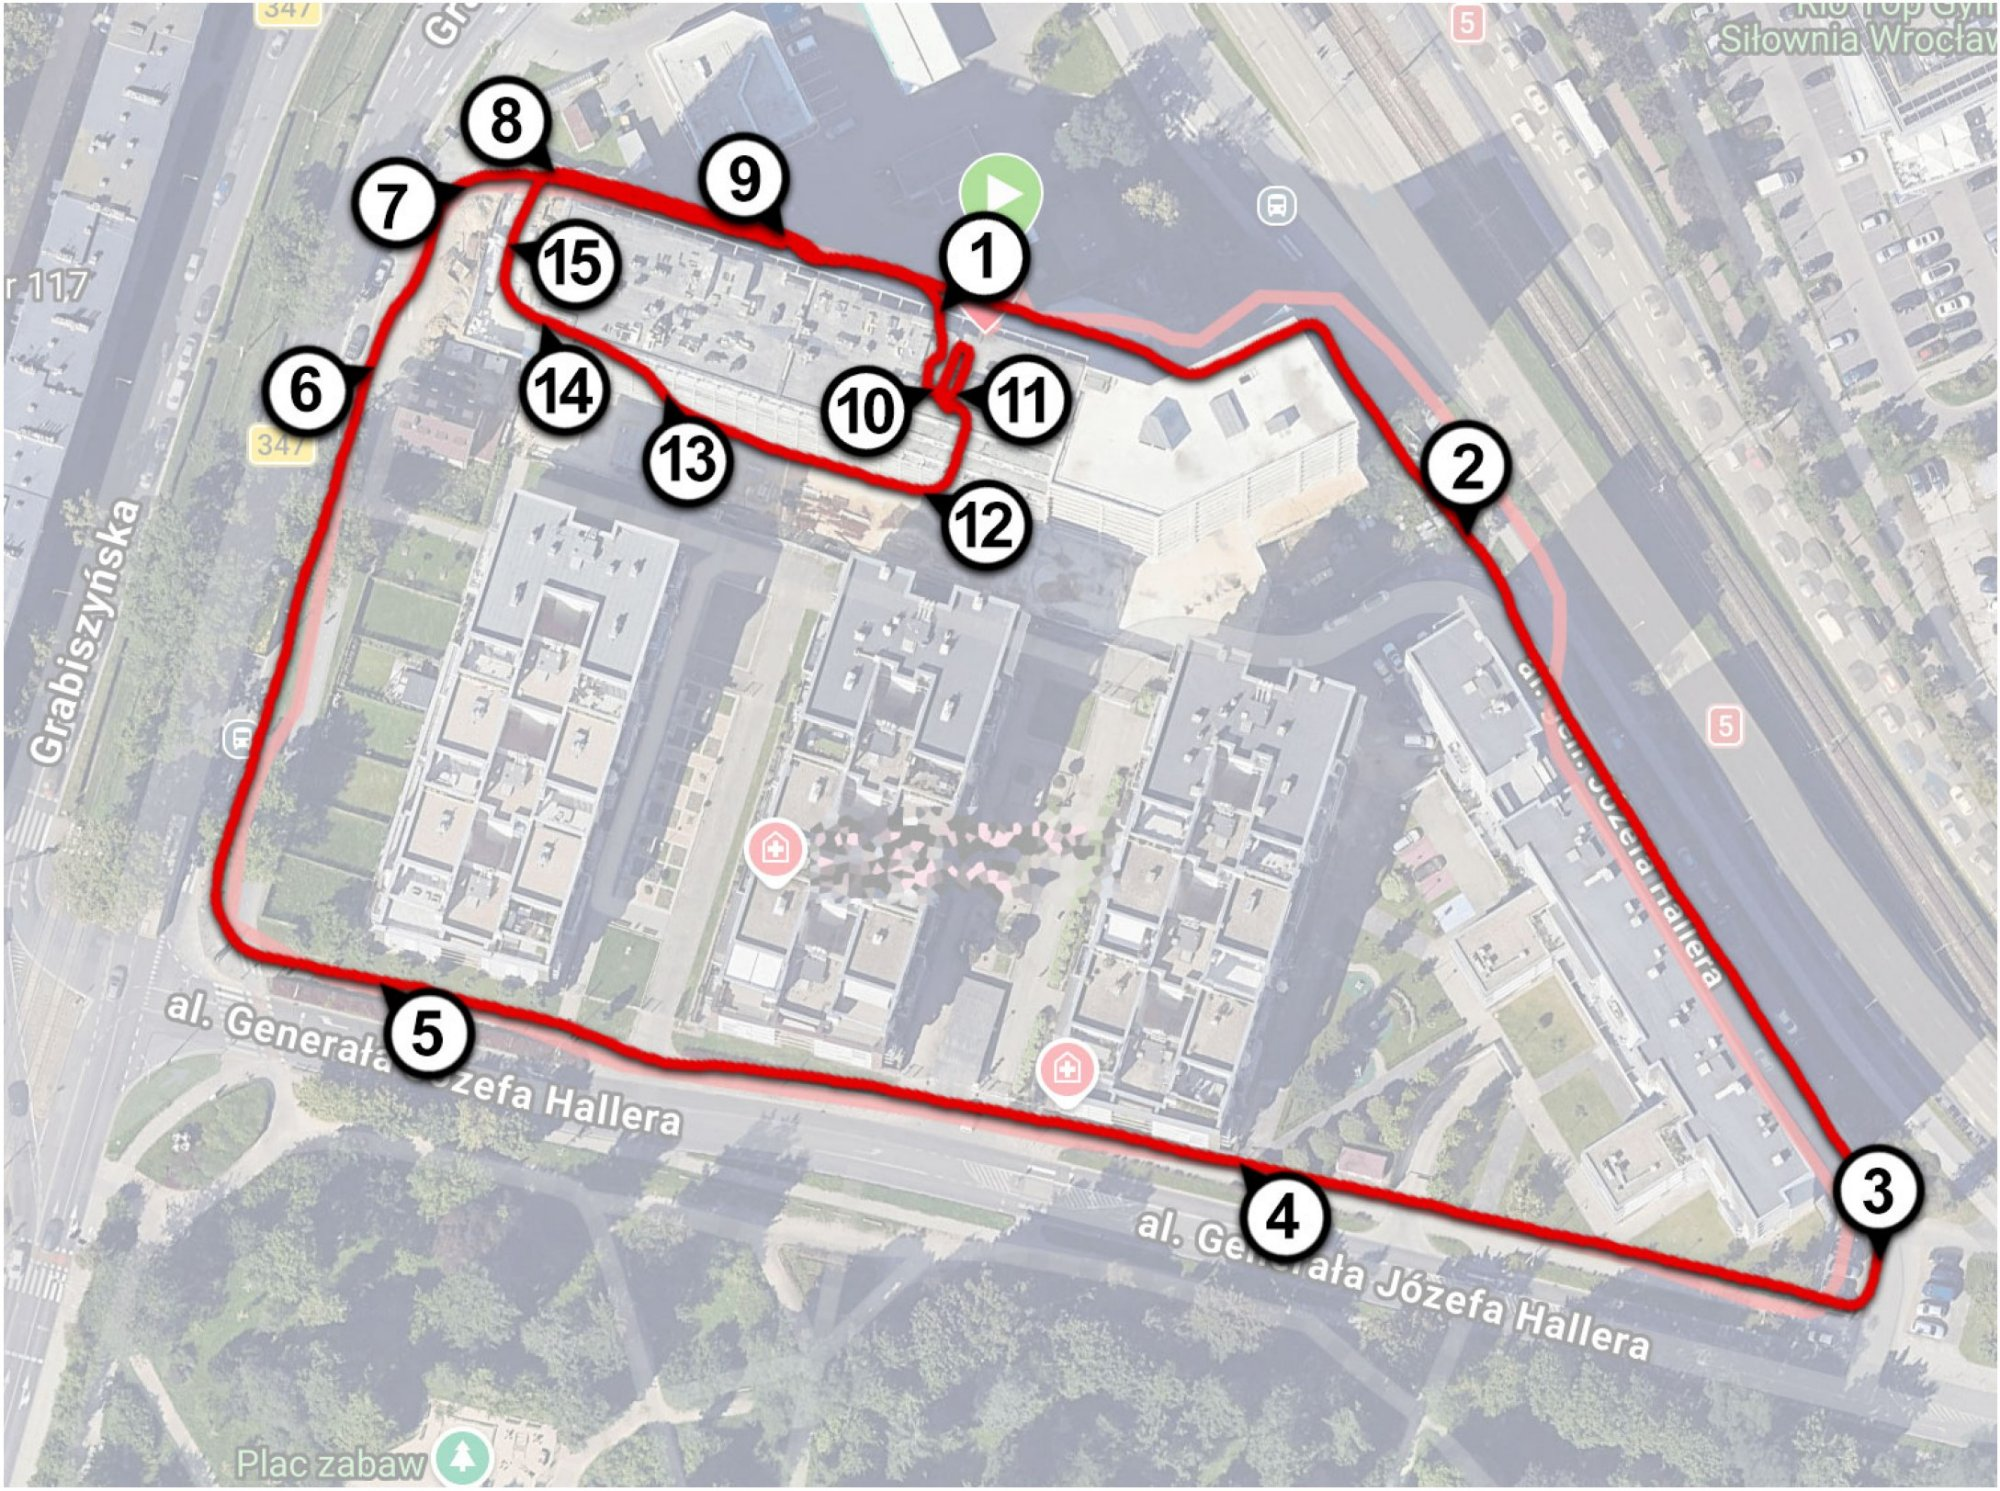
\includegraphics[width=\textwidth]{fig_route_map.jpg}
\caption{Satellite overlay of the test route at Al.~Hallera~204, Wroc\l{}aw.
Red trace shows a GPS recording from a Garmin watch (outdoor segments only;
three separate days were averaged to establish ground truth). Numbered markers
(1--15) correspond to the waypoint photographs in Fig.~\ref{fig:route_photos}.
The route forms a closed loop of approximately 600\,m per circuit, with
${\sim}40$\% underground.}
\label{fig:route_map}
\end{figure}

\begin{figure}[H]
\centering
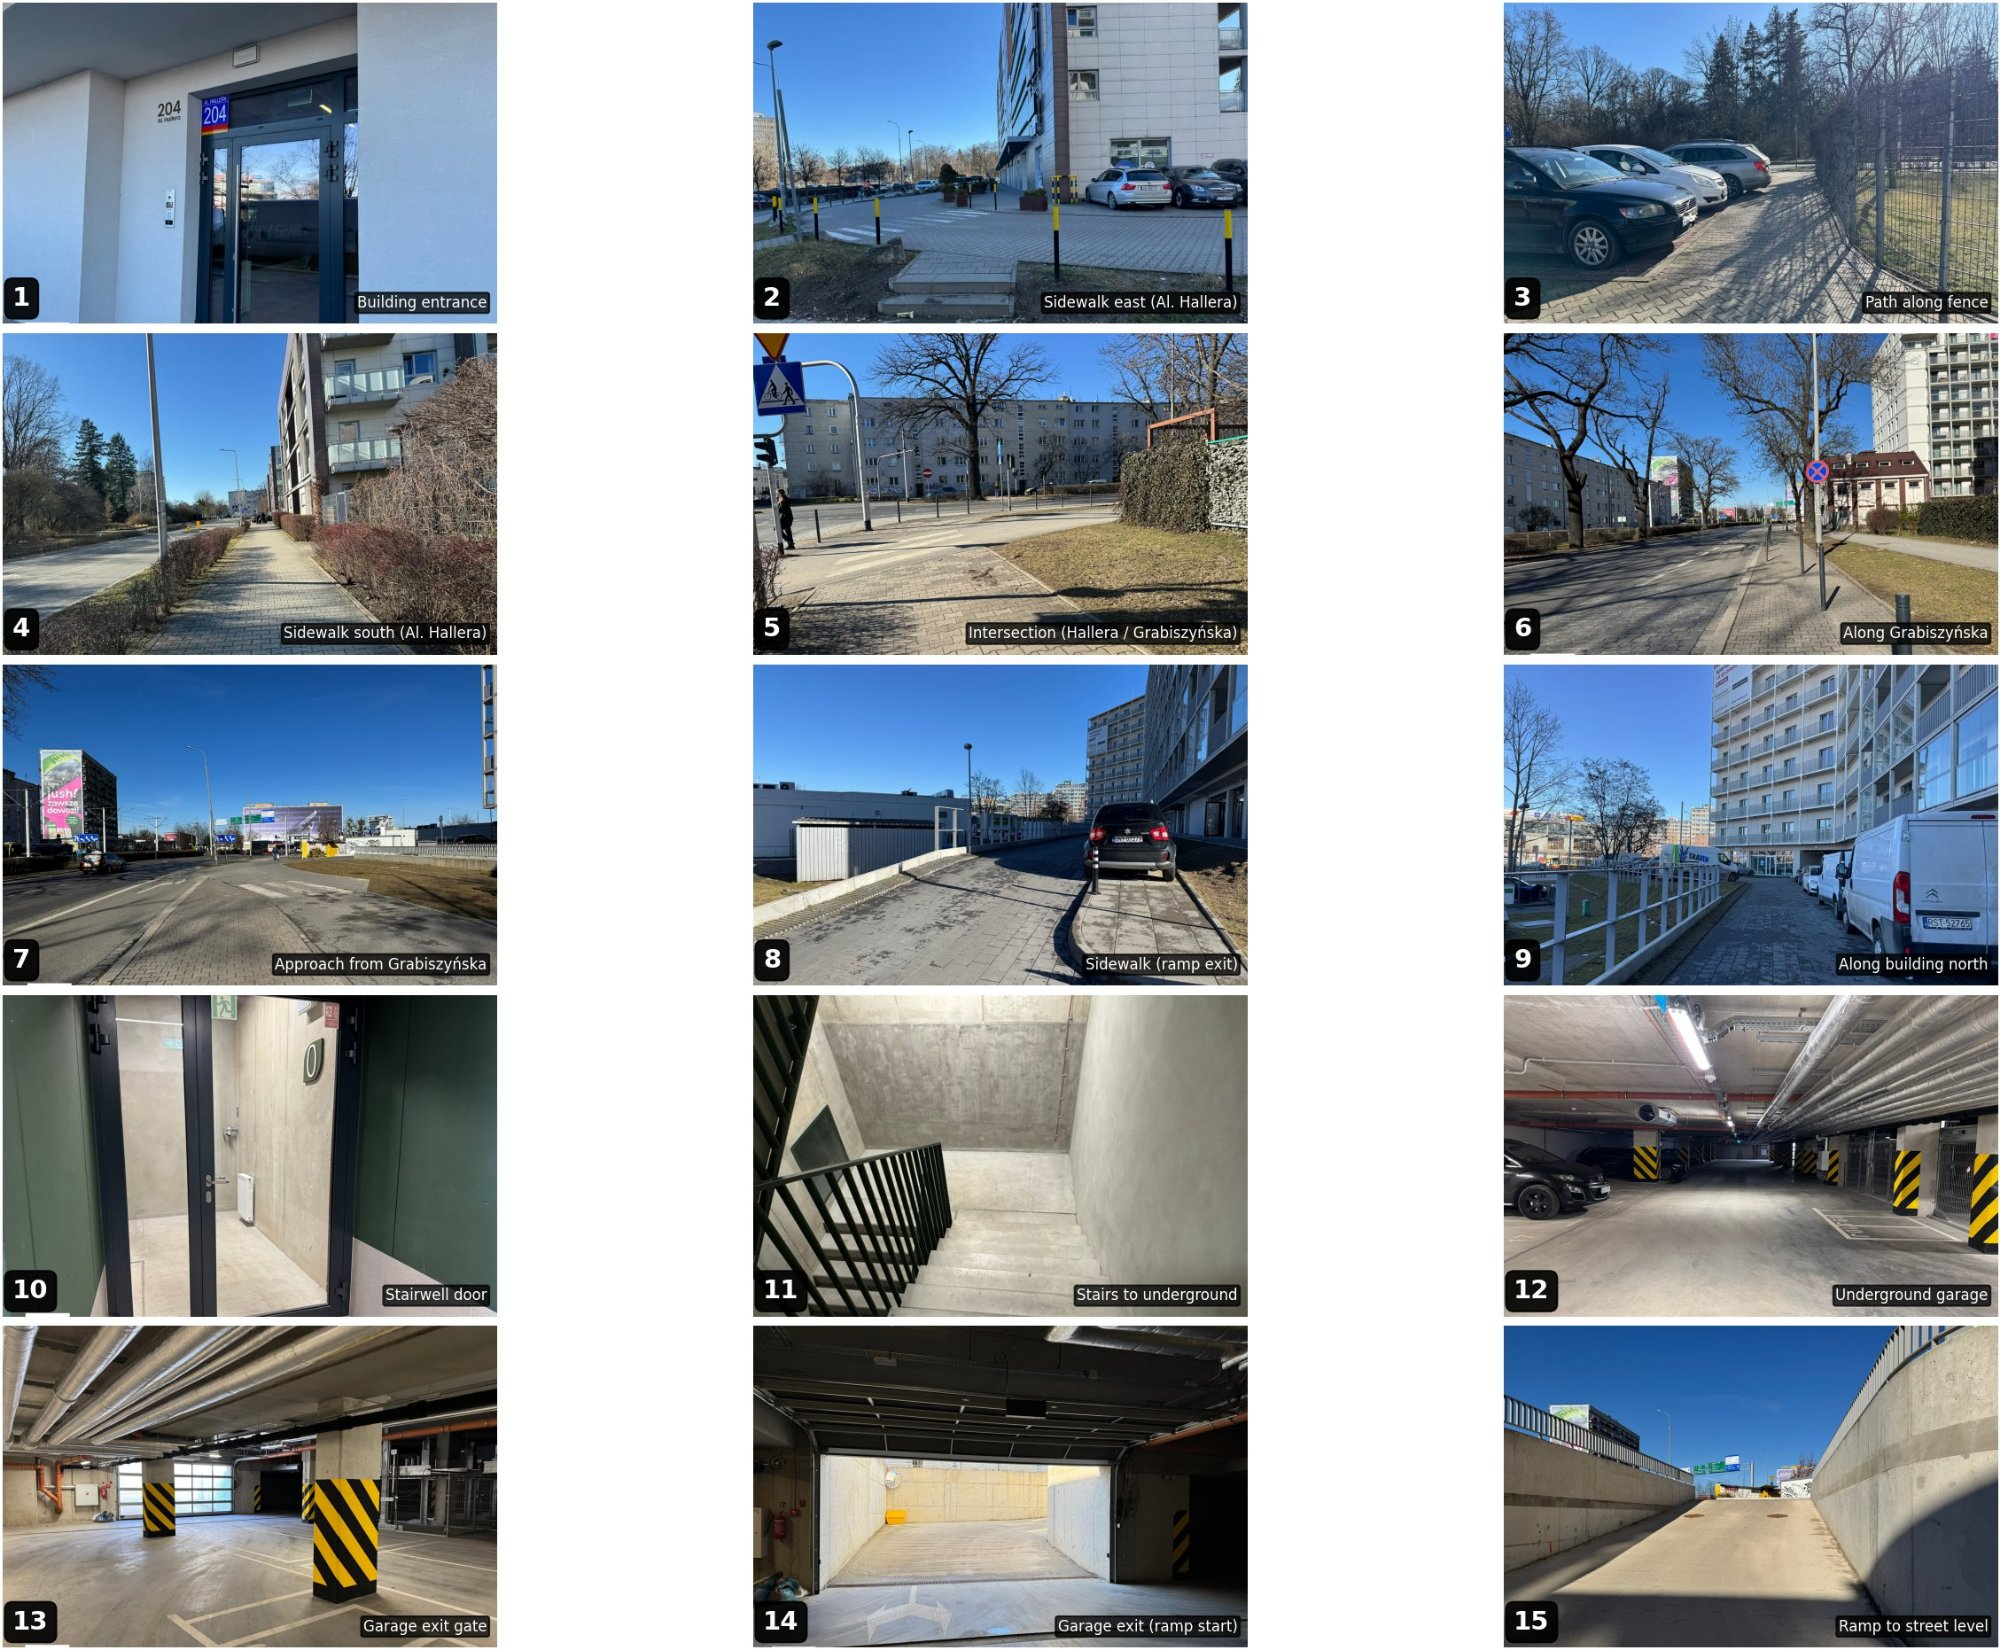
\includegraphics[width=\textwidth]{fig_route_photos.jpg}
\caption{Photographs at each of the 15 waypoints marked in
Fig.~\ref{fig:route_map}. Outdoor segment: sidewalks and intersection (1--9).
Indoor segment: stairwell (10--11), underground garage with reinforced concrete
and metal ducting (12--13), vehicle ramp exit (14--15). The variety of terrain,
lighting, and magnetic environment represents conditions under which GPS and
magnetometer-based systems would fail or require recalibration.}
\label{fig:route_photos}
\end{figure}

\subsection{Recording Protocol}

Four recordings were collected from one healthy male (170\,cm, 70\,kg) across
12 days (January 24--February 4, 2026). No calibration walk was performed. No
magnetometer was used. The subject walked at self-selected brisk pace.

Recording~C included a simultaneous Garmin Approach~S70 GPS track for outdoor
segments and followed a structured route: three outdoor loops around a city
block alternating with three indoor garage loops. The GPS ground truth for the
outdoor loop (640\,m) was established by three prior independent GPS walks.

\subsection{Closure Methodology}

All walks were closed loops returning to the starting position. Closure error
is computed as the Euclidean distance between the first and last points of the
reconstructed path, expressed as a percentage of total distance walked.

Closure percentage is $K$-independent: the calibration constant $K$ scales
total distance and final displacement equally, so path shape (and therefore
closure percentage) is identical regardless of how $K$ is estimated. This
means the closure results hold for any subject height or calibration method.

% ====================================================================
\section{Results}
\label{sec:results}

\subsection{Summary}

\begin{table}[H]
\centering
\caption{PDR Results: Four Independent Recordings}
\label{tab:results}
\begin{tabular}{@{}ccrcccccc@{}}
\toprule
Rec. & Date & Dist. & Clos. & Clos. & $\sigma_\psi$ & NZ $\sigma$ & Cad. & Steps \\
     &      & (m)   & (m)   & (\%)  & (\textdegree) & (\textdegree) & (spm) & \\
\midrule
A & Jan\,24 & 2138 & 10.4 & 0.49 & 7.81 & 1.87 & 127 & 3321 \\
B & Feb\,1  & 2428 & 4.3  & 0.18 & 7.22 & 1.82 & 124 & 3782 \\
C & Feb\,2  & 2339 & 13.7 & 0.58 & 8.53 & 1.93 & 123 & 3643 \\
D & Feb\,4  & 2407 & 23.0 & 0.95 & 7.65 & 1.79 & 122 & 3737 \\
\midrule
\multicolumn{2}{c}{\textbf{Mean}} & \textbf{2328} & 12.9 & \textbf{0.55} & 7.80 & 1.85 & 124 & 14483 \\
\bottomrule
\end{tabular}
\end{table}

Mean closure: \textbf{0.55\%} across 9.3\,km and 14,483 steps. All four
recordings achieve sub-1\% closure over multi-kilometer distances.

\subsection{Per-Recording Detailed Analysis}

Figures~\ref{fig:runA}--\ref{fig:runD} present the complete diagnostic panels
for each recording. Each figure contains six sub-panels:

\begin{enumerate}[nosep]
\item \textbf{PDR Path} (top left): Reconstructed trajectory with terrain
coloring (blue = level, red = uphill, light blue = downhill). Green circle =
start, red star = end.
\item \textbf{Panjabi Neutral Zone} (top right): 2D pitch--roll histogram with
hub position (cyan star). The tight, unimodal distribution confirms stable
neutral zone identification.
\item \textbf{NZ Terrain Detection} (middle left): Nadir pitch offset from hub
over time. Uphill/downhill thresholds shown. Terrain segments match known
garage ramp positions.
\item \textbf{Stride Histogram} (middle right): Distribution of stride
lengths with mean and standard deviation.
\item \textbf{Per-Step Heading} (bottom left): Individual step heading changes
$\Delta\psi$. Mean near zero with $\sigma \approx 7$--8.5\textdegree.
\item \textbf{Random Walk Test} (bottom right): Cumulative heading with
$\pm\sigma\sqrt{n}$ envelope. If per-step errors are independent, cumulative
heading should stay within this envelope---and it does in all recordings.
\end{enumerate}

% --- Recording A ---
\begin{figure}[p]
\centering
\includegraphics[width=\textwidth]{run1.png}
\caption{\textbf{Recording~A} (January 24): 2138\,m, 3321 steps, closure
10.4\,m (\textbf{0.49\%}). Per-step heading $\sigma = 7.8$\textdegree.
Cumulative heading stays within $\pm\sigma\sqrt{n}$ random walk bounds. Hub
pitch: 77.4\textdegree, NZ spread: 1.87\textdegree. Stride:
$0.644 \pm 0.323$\,m. Terrain detection identifies 136 uphill and 81
downhill steps matching garage ramp geometry.}
\label{fig:runA}
\end{figure}

% --- Recording B ---
\begin{figure}[p]
\centering
\includegraphics[width=\textwidth]{run4.png}
\caption{\textbf{Recording~B} (February 1): 2428\,m, 3782 steps, closure
4.3\,m (\textbf{0.18\%}). Best result. Per-step heading $\sigma =
7.2$\textdegree{} (lowest). Hub pitch: 76.1\textdegree, NZ spread:
1.82\textdegree. Stride: $0.642 \pm 0.323$\,m. Terrain: 148 uphill, 107
downhill steps. Random walk test shows cumulative heading tightly bounded near
zero throughout. The 0.18\% closure demonstrates that sub-degree heading
accuracy is achievable from spine-mounted IMU.}
\label{fig:runB}
\end{figure}

% --- Recording C ---
\begin{figure}[p]
\centering
\includegraphics[width=\textwidth]{run2.png}
\caption{\textbf{Recording~C} (February 2): 2339\,m, 3643 steps, closure
13.7\,m (\textbf{0.58\%}). This is the GPS cross-validated recording.
Per-step heading $\sigma = 8.5$\textdegree{} (highest, reflecting the more
complex mixed indoor--outdoor route). Hub pitch: 78.6\textdegree, NZ spread:
1.92\textdegree. Stride: $0.642 \pm 0.311$\,m. Terrain: 236 uphill, 125
downhill steps (more terrain variation due to outdoor segments with
inclines).}
\label{fig:runC}
\end{figure}

% --- Recording D ---
\begin{figure}[p]
\centering
\includegraphics[width=\textwidth]{run3.png}
\caption{\textbf{Recording~D} (February 4): 2407\,m, 3737 steps, closure
23.0\,m (\textbf{0.95\%}). Weakest result, but still sub-1\%. Per-step heading
$\sigma = 7.7$\textdegree. Hub pitch: 80.9\textdegree{} (highest, suggesting
slight sensor placement shift). NZ spread: 1.79\textdegree{} (tightest).
Stride: $0.644 \pm 0.327$\,m. Random walk test shows cumulative heading
excursion approaching the $\pm\sigma\sqrt{n}$ envelope boundary around step
2500, contributing to the higher closure error.}
\label{fig:runD}
\end{figure}

\subsection{Neutral Zone Stability}

\begin{table}[H]
\centering
\caption{Neutral Zone Hub Consistency Across 12 Days}
\label{tab:nz}
\begin{tabular}{@{}ccccc@{}}
\toprule
Recording & Hub Pitch (\textdegree) & Hub Roll (\textdegree) & NZ Spread $\sigma$ (\textdegree) & K \\
\midrule
A & 77.4 & $-$3.2 & 1.87 & 0.3604 \\
B & 76.1 & $-$2.1 & 1.82 & 0.4680 \\
C & 78.6 & $-$4.8 & 1.92 & 0.4161 \\
D & 80.9 & $-$2.4 & 1.79 & 0.4279 \\
\midrule
\textbf{Mean} & \textbf{78.3} & $-$\textbf{3.1} & \textbf{1.85} & --- \\
\textbf{SD} & \textbf{2.0} & \textbf{1.2} & \textbf{0.06} & --- \\
\bottomrule
\end{tabular}
\end{table}

The NZ spread is stable at $1.85 \pm 0.06$\textdegree{} across 12 days.
The pitch variation (2.0\textdegree{} SD) likely reflects day-to-day sensor
placement differences. The NZ spread itself---the \textit{width} of the
neutral zone, not its position---varies by only 0.06\textdegree, indicating a
highly reproducible biomechanical property. This is the first continuous
measurement of Panjabi's Neutral Zone spread in a living person.

\subsection{GPS Cross-Validation}
\label{sec:gps}

Recording~C followed a structured protocol: three outdoor loops around a city
block alternating with three indoor garage loops. Ground truth for the outdoor
loop was established by three prior walks with a Garmin Approach~S70 GPS watch
(mean 640\,m per loop).

\begin{figure}[H]
\centering
\includegraphics[width=0.85\textwidth]{fig_2.png}
\caption{Recording~C: PDR paths overlaid on satellite imagery (Wroc\l{}aw,
Poland). Red: Garmin Approach~S70 GPS ground truth. Blue: NimBrace PDR.
Orange: uphill segments. Yellow: downhill segments. Green circle: start; red
star: end. The PDR tracks align with actual sidewalks and building perimeters,
confirming heading accuracy. Indoor garage loops (blue, upper portion) are
invisible to GPS.}
\label{fig:gps}
\end{figure}

\begin{table}[H]
\centering
\caption{Recording~C: GPS Cross-Validation}
\label{tab:gps}
\begin{tabular}{@{}lcrrr@{}}
\toprule
Segment & Type & Steps & PDR (m) & GPS (m) \\
\midrule
Outdoor Ring 1 & outdoor & 900 & 581 & 640 \\
Garage Loop 1  & indoor  & 310 & 179 & --- \\
Outdoor Ring 2 & outdoor & 876 & 600 & 640 \\
Garage Loop 2  & indoor  & 304 & 181 & --- \\
Outdoor Ring 3 & outdoor & 877 & 594 & 640 \\
Garage Loop 3  & indoor  & 375 & 205 & --- \\
\midrule
Outdoor total  & outdoor & 2653 & 1774 & 1920 \\
Indoor total   & indoor  & 989 & 565 & --- \\
\bottomrule
\end{tabular}

\vspace{2mm}
{\footnotesize PDR distances use default height (1.70\,m). The 8\% outdoor
underestimate reflects the allometric formula assuming average gait speed while
the subject walked briskly.}
\end{table}

\textbf{Reproducibility.} Three independent PDR measurements of the same
outdoor loop: 581, 600, 594\,m (mean $591 \pm 8$\,m, CV = 1.3\%). This
internal consistency---three passes without calibration---demonstrates reliable
measurement of a stable biomechanical property.

\textbf{GPS calibration transfer.} Using GPS outdoor distance to calibrate
$K$: outdoor total becomes 1929\,m vs.\ GPS ground truth 1920\,m (+0.4\%
error), confirming stride proxy linearity across environments.
GPS-calibrated indoor garage loops: 195, 197, 222\,m per loop---distances
inaccessible to satellite navigation, now derived with GPS-validated
calibration.

\textbf{Height sensitivity.} The GPS-calibrated $K$ implies step length of
0.694\,m, consistent with the allometric formula for a taller subject
(${\sim}$1.85\,m). The actual subject (1.70\,m) was walking briskly,
confirming that the allometric coefficient (0.375) assumes average gait speed.
For clinical use where absolute distance matters, a short GPS calibration walk
can eliminate height dependence entirely.

% ====================================================================
\section{Comparison with Prior Art}
\label{sec:comparison}

\begin{table}[H]
\centering
\caption{Comparison with Published PDR Systems}
\label{tab:comparison}
\begin{tabular}{@{}lccccc@{}}
\toprule
System & Mount & Heading Method & Mag. & Dist. & Closure \\
\midrule
Foxlin~\cite{foxlin2005}         & foot  & compass         & yes & 0.7\,km    & $\sim$0.3\% \\
Nilsson~\cite{nilsson2012}       & foot  & uncontrolled    & no  & var.       & 1--2\% \\
Skog~\cite{skog2010}             & foot  & ZUPT only       & no  & var.       & 1--2\% \\
Borenstein~\cite{borenstein2010} & waist & HDE             & no  & $<$1\,km   & 2--3\% \\
Beauregard~\cite{beauregard2006} & waist & magnetometer    & yes & $<$0.5\,km & 3--5\% \\
Jimenez~\cite{jimenez2009}       & waist & mag + HDE       & yes & $<$0.5\,km & 5--8\% \\
Lu~\cite{lu2019}                 & chest & mag + map       & yes & $<$1\,km   & $\sim$5\,m \\
\textbf{This work}               & \textbf{spine} & \textbf{Zero-Cycle} & \textbf{no} & \textbf{9.3\,km} & \textbf{0.55\%} \\
\bottomrule
\end{tabular}

\vspace{2mm}
{\footnotesize ZUPT corrects velocity/position but heading error is
unobservable~\cite{nilsson2012}. HDE = Heuristic Drift Elimination (assumes
orthogonal building corridors).}
\end{table}

The heading method column reveals the central problem in PDR: ZUPT bounds
velocity drift but leaves heading unobservable. Every prior system without
magnetometer relies on external constraints (building geometry, GPS) for
heading. Zero-Cycle is the first approach that solves heading drift through
biomechanical synchronization alone---no magnetometer, no building model, no
infrastructure.

The 0.55\% mean closure across 9.3\,km represents an order-of-magnitude
improvement over prior torso-mounted systems (3--8\%) and matches or exceeds
foot-mounted ZUPT performance (1--2\%). Notably, this is achieved at distances
far exceeding any prior work: the longest individual recording (B, 2428\,m) is
$3\times$ the distance of most published PDR evaluations.

% ====================================================================
\section{Discussion}
\label{sec:discussion}

\subsection{Why Zero-Cycle Works}

Where ZUPT solves the velocity problem (making position error grow as
O($\sqrt{n}$) instead of O($n^2$)), Zero-Cycle solves the heading problem
(making heading error grow as O($\sqrt{n}$) instead of O($n$)). These are
complementary solutions to orthogonal error sources. Together, ZUPT and
Zero-Cycle bound both fundamental PDR error sources---but Zero-Cycle does not
require foot mounting.

The BNO085 game rotation vector uses internal sensor fusion: gyroscope for fast
rotation tracking and accelerometer for gravity reference (pitch/roll). At
nadir points (minimum angular velocity), the internal filter has maximum
confidence in its gravity correction. This means the quaternion output is most
stable exactly when Zero-Cycle samples it---a happy synergy between the
biomechanical principle and the sensor's internal algorithm.

\subsection{The Nadir Advantage}

The nadir principle represents a conceptual shift from global to local
references. By using the local minimum-energy configuration---Panjabi's
Neutral Zone~\cite{panjabi1992} made operational---the algorithm handles
terrain without mode switching. This is why nadir heading reduces closure from
1.47\% to 0.71\% compared to hub crossings (Recording~B, same stride method)
while recovering 99.9\% vs.\ 53\% of steps.

The nadir is also inherently a better sampling point than a heel strike. At
heel strike, the sensor experiences a high-amplitude vibration transient
($>$5\,g at the foot, attenuated but still present at T4). At nadir, the
sensor is at its minimum angular velocity---the smoothest, most stable point in
the gait cycle.

\subsection{The Biomechanical Ruler}

The 35\,cm T4--S1 inter-sensor spacing provides physical grounding absent from
single-IMU estimators. The differential acceleration captures thoracopelvic
counter-rotation, spine compression during impact, and lateral bending during
weight transfer---biomechanically meaningful quantities that are insensitive to
whole-body motion via common-mode rejection.

Higher per-step variability (CV = 0.52) paradoxically improves path accuracy
because it tracks genuine stride variation. The spine deforms differently
during turns (more lateral bending), straight segments (sagittal dominance),
and speed changes (variable impact), and the differential signal captures
these differences.

\subsection{Dual-Use Capability}

The dual-IMU spine configuration simultaneously provides navigation capability
(heading, stride, terrain) and clinical measurement (flexion/extension, lateral
bending, axial rotation). The NimBrace device was developed for continuous
spine biomechanical monitoring; indoor navigation emerges as a dual-use
capability from the same hardware and data stream.

\subsection{Generalizability}

The Zero-Cycle principle requires only periodic motion returning to a
minimum-energy configuration. While validated here for gait (pelvis nadir at
each step), the same principle should generalize to any cyclic body
segment---knee flexion/extension during walking, hip rotation, ankle
dorsiflexion, shoulder abduction during repetitive tasks---wherever the joint
parks at a biomechanically defined neutral state between movement cycles.

\subsection{Limitations}

Testing was performed on a single healthy subject; pathological gait needs
validation. The inter-sensor spacing varies with body habitus. Recording~D
achieved the weakest closure (0.95\%), with hub pitch 80.9\textdegree{}
(vs.\ 76.1--78.6\textdegree{} for others), suggesting day-to-day sensor
placement variability warrants investigation. The 8\% stride underestimate
when using default height (1.70\,m) indicates that allometric scaling alone is
insufficient for subjects with non-average gait speed; a short GPS calibration
walk resolves this.

% ====================================================================
\section{Conclusion}
\label{sec:conclusion}

Nadir-based Zero-Cycle heading---the first biomechanical solution to IMU
heading drift---and differential accelerometry achieve mean 0.55\% closure from
spine-mounted dual IMU across 9.3\,km without magnetometer. Where ZUPT bounds
velocity drift, Zero-Cycle bounds heading drift; together they solve both
fundamental PDR error sources. The system recovers 99.9\% of steps (vs.\ 53\%
for hub crossings), classifies terrain from neutral zone pitch shift, and is
cross-validated against GPS at 0.4\% outdoor distance error. The principle
generalizes to any cyclic body segment with a biomechanically defined neutral
state. The spine, parking at its Neutral Zone every step, provides both
navigation reference and clinical signal.

\section*{Data and Code Availability}

Complete source code and raw data files are available at:\\
\url{https://github.com/gmiekisiak/spinerebel}

% ====================================================================
\begin{thebibliography}{14}

\bibitem{panjabi1992}
M.~M.~Panjabi, ``The stabilizing system of the spine. Part~I: Function,
dysfunction, adaptation, and enhancement,'' \textit{J.\ Spinal Disord.},
vol.~5, no.~4, pp.~383--389, 1992.

\bibitem{foxlin2005}
E.~Foxlin, ``Pedestrian tracking with shoe-mounted inertial sensors,''
\textit{IEEE Comput.\ Graph.\ Appl.}, vol.~25, no.~6, pp.~38--46, 2005.

\bibitem{beauregard2006}
S.~Beauregard and H.~Haas, ``Pedestrian dead reckoning: A basis for personal
positioning,'' in \textit{Proc.\ 3rd Workshop Positioning, Navig.\ Commun.},
2006, pp.~27--35.

\bibitem{weinberg2002}
H.~Weinberg, ``Using the ADXL202 in pedometer and personal navigation
applications,'' Analog Devices, Appl.\ Note AN-602, 2002.

\bibitem{oberg1993}
K.~\"{O}berg, A.~Karsznia, and K.~\"{O}berg, ``Basic gait parameters:
Reference data for normal subjects, 10--79 years of age,'' \textit{J.\
Rehabil.\ Res.\ Dev.}, vol.~30, pp.~210--223, 1993.

\bibitem{bno085}
\textit{BNO085 Datasheet}, CEVA/Hillcrest Labs, 2021.

\bibitem{moenilssen2004}
R.~Moe-Nilssen and J.~L.~Helbostad, ``Estimation of gait cycle
characteristics by trunk accelerometry,'' \textit{J.\ Biomech.}, vol.~37,
no.~1, pp.~121--126, 2004.

\bibitem{sola2017}
J.~Sol\`{a}, ``Quaternion kinematics for the error-state Kalman filter,''
\textit{arXiv:1711.02508}, 2017.

\bibitem{jimenez2009}
A.~R.~Jimenez \textit{et al.}, ``A comparison of pedestrian dead-reckoning
algorithms using a low-cost MEMS IMU,'' in \textit{Proc.\ IEEE WISP}, 2009,
pp.~37--42.

\bibitem{skog2010}
I.~Skog \textit{et al.}, ``Zero-velocity detection---An algorithm evaluation,''
\textit{IEEE Trans.\ Biomed.\ Eng.}, vol.~57, no.~11, pp.~2657--2666, 2010.

\bibitem{nilsson2012}
J.-O.~Nilsson, I.~Skog, and P.~H\"{a}ndel, ``A note on the limitations of
ZUPTs and the implications on sensor error modeling,'' in \textit{Proc.\ IEEE
IPIN}, Sydney, Australia, 2012.

\bibitem{borenstein2010}
J.~Borenstein and L.~Ojeda, ``Heuristic drift elimination for personnel
tracking systems,'' \textit{J.\ Navig.}, vol.~63, no.~4, pp.~591--606, 2010.

\bibitem{lu2019}
C.~Lu \textit{et al.}, ``Indoor positioning system based on chest-mounted
IMU,'' \textit{Sensors}, vol.~19, no.~2, p.~420, 2019.

\bibitem{miekisiak2026letter}
G.~Miekisiak, ``Torso-mounted pedestrian dead reckoning using nadir-based
zero-cycle heading and differential accelerometry,'' \textit{IEEE Sensors
Lett.}, submitted, 2026.

\end{thebibliography}

\end{document}
